\chapter{Über Kojo}
\begin{multicols}{2}
\section*{\color{black}Was ist Kojo?}
Kojo ist eine App die hilfen Sie programmieren zu lernen. Mit Kojo, Sie können in der modernen und leistungsfähigen Programmiersprache {\bf\color{blue}Scala} kodieren. Kojo ist kostenlos und gibt auf Deutsch. Kojo funktioniert mit Linux, Windows und Mac OSX.
\section*{\color{black}Wo finde ich Kojo?}
Download Kojo: 
\href{http://www.kogics.net/kojo-download}{www.kogics.net/kojo-download}
Lesen Sie hier mehr: 
\href{http://lth.se/programmera}{lth.se/programmera}

\columnbreak

\begin{center}
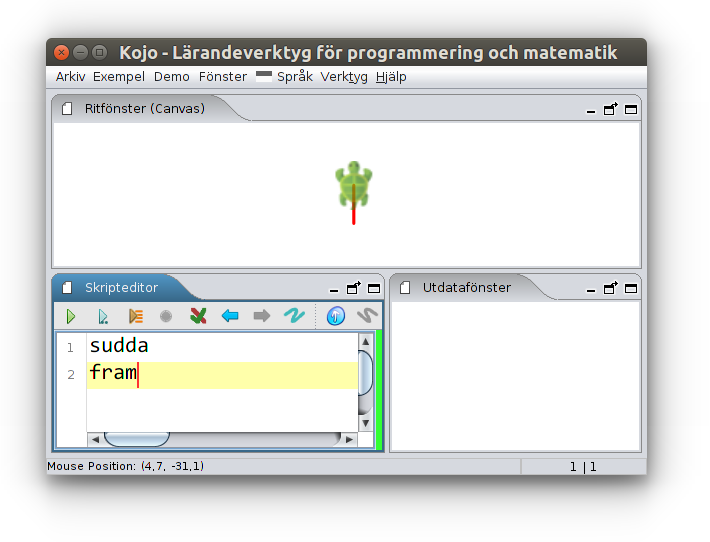
\includegraphics{../img/kojo.png}
\end{center}

\end{multicols}

\chapter{Ihr erstes Programm}
\begin{multicols}{2}

\begin{lstlisting}[basicstyle={\ttfamily\fontsize{36.0}{36.0}\selectfont}]
clear
forward
\end{lstlisting}
        
Drücken Sie die grüne Play-Taste um kick off Programm.

\columnbreak

\begin{center}
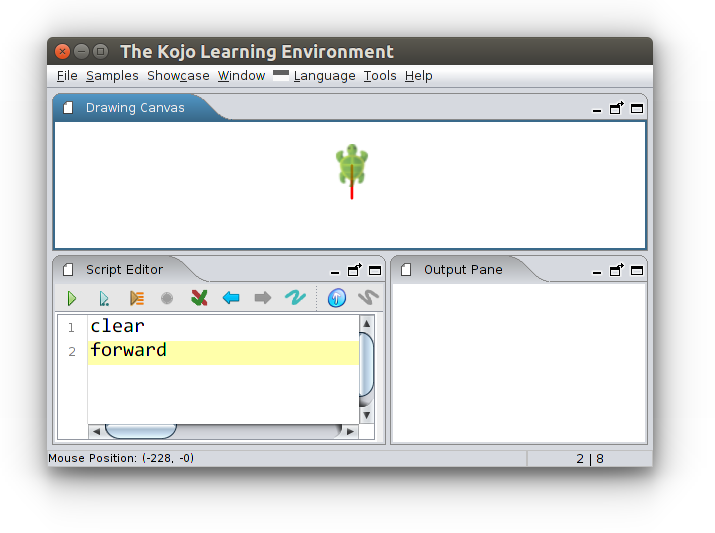
\includegraphics[width=14.0cm]{../img/forward.png}
\end{center}

\end{multicols}

